\chapter{Project Methodology}
 \section{Software Development Model}
 The Agile model is an adaptable and iterative software development process that puts the needs of the client and flexibility first. It breaks the project up into manageable chunks known as sprints or iterations, enabling regular review and modification. Close collaboration between cross-functional teams results in functional software at the conclusion of each iteration. This cycle of iteration guarantees prompt reaction to evolving needs, promoting ongoing enhancement and contentment for the client. The Agile Manifesto's concepts of agile development include a strong emphasis on people and their relationships, functional software, customer collaboration, and adapting to change. In dynamic development contexts, the Agile approach has gained widespread adoption as a framework that encourages efficiency and reactivity.
 \begin{figure}[h]
	\centering
	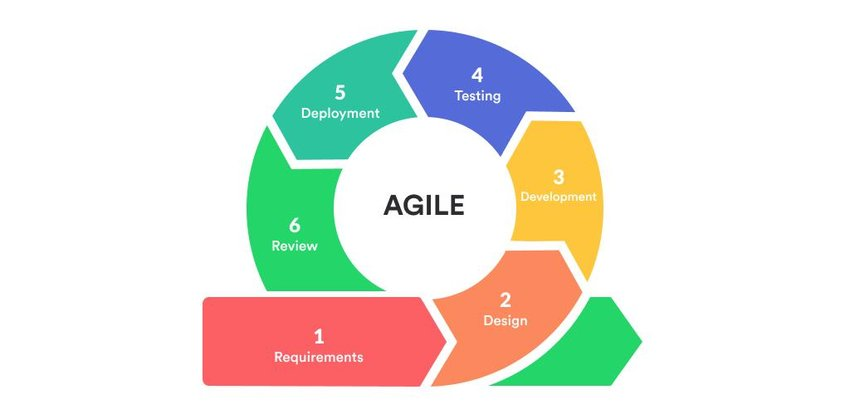
\includegraphics[scale=0.6]{images/Agile_model.png}
	\caption{Agile Model}
	
	\end{figure}
	
\pagebreak
\section{Block Diagram of proposed system}
	\begin{figure}[h]
		\centering
		\hspace{2cm}
		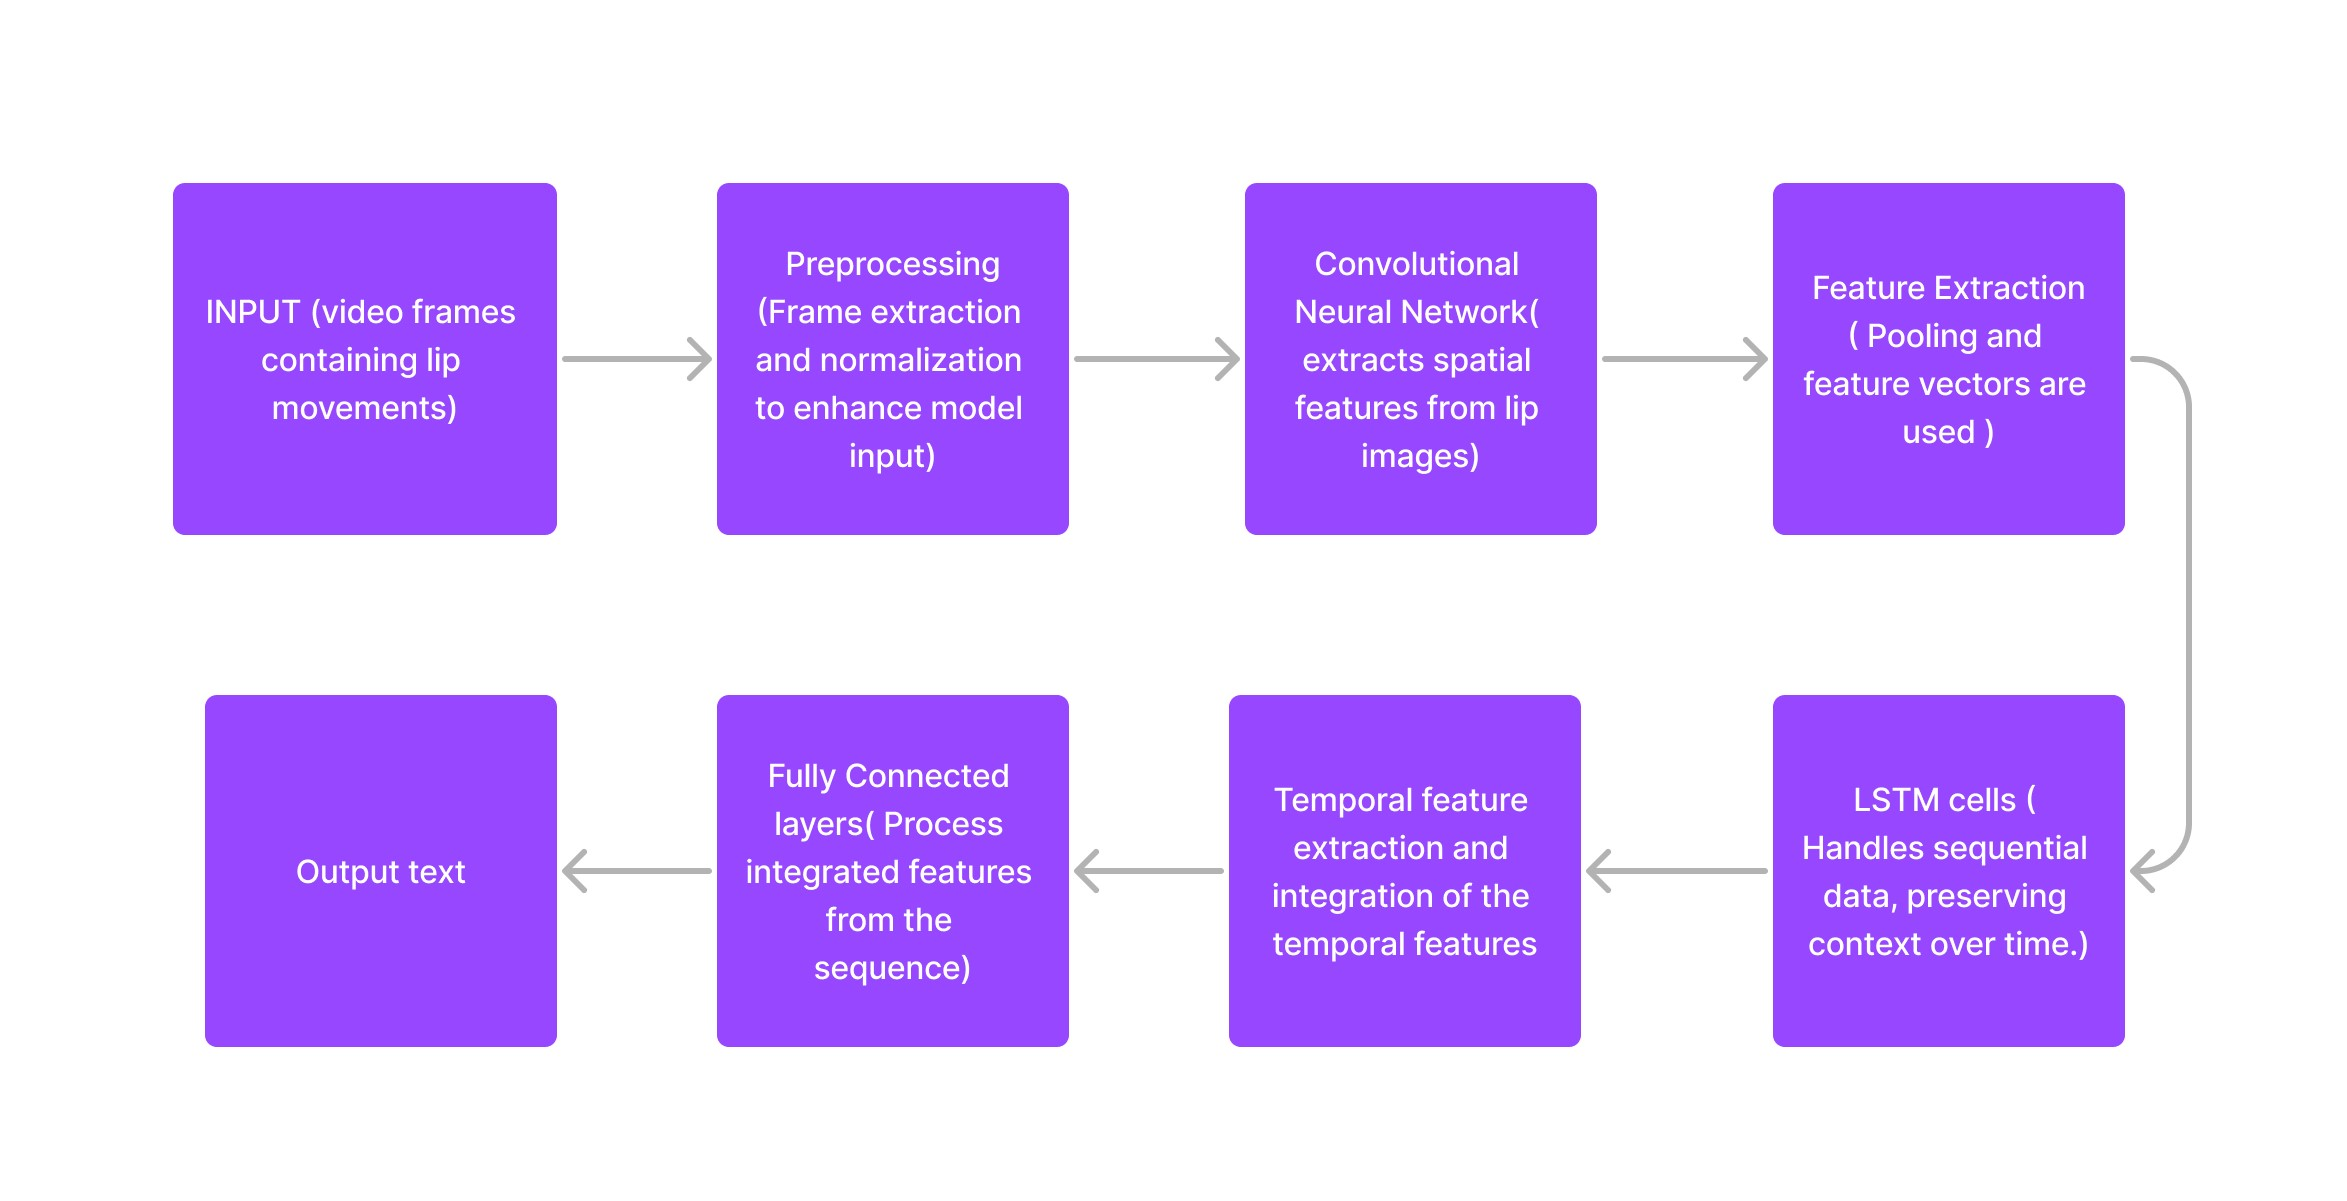
\includegraphics[scale=0.35]{images/block_diagram.jpg}
		\caption{Block Diagram of Proposed System}
	\end{figure}
	
	
	

\section{Description of working flow of proposed system}
\begin{enumerate}
	\item \textbf{Input(Video Frames):}
	\\ The system takes video frames containing lip movements as input, forming the basis for lip reading analysis.
	\item \textbf{Preprocessing:}
	\\Frames undergo extraction and normalization to enhance the model's input quality, ensuring consistent and standardized input data.
	\item \textbf{Convolutional Neural Network (CNN):}
	\\A CNN is employed to extract spatial features from lip images by utilizing convolutional layers with filters. These filters detect spatial patterns within the lip movements.
	\item \textbf{Feature Extraction:}
	\\Pooling layers are used to reduce spatial dimensions, and the result is feature vectors that effectively represent distinctive lip features.
	\item \textbf{Recurrent Neural Network (RNN):}
	\\RNN processes temporal sequences of features, allowing the model to capture temporal dependencies within the lip movements.
	\item \textbf{Long Short-Term Memory (LSTM) Cells}
	\\Specialized LSTM cells are incorporated to handle sequential data, preserving context over time and enhancing the model's ability to understand the temporal aspects of lip movements.
	\item \textbf{Temporal Feature Extraction:}
	\\The model extracts temporal features from the sequential data, contributing to a more comprehensive understanding of the temporal dynamics of lip motion.
	\item \textbf{Integration Layer:}
	\\An integration layer merges both spatial and temporal features, creating a unified representation that combines information from different aspects of the input data.
	\item \textbf{Fully Connected Layers:}
	\\These layers process the integrated features for classification, preparing the data for the final prediction stage.
	\item \textbf{Output (Text Prediction):}
	\\The final layer of the model predicts the corresponding text or phonemes based on the processed spatial and temporal features.
\end{enumerate}